%!TEX root=description_of_changed_files.tex

\section{fixes}

\subsection{fix\_active\_fluct}


\subsection{fix\_bond\_create\_break}

This fix introduces the bond formation and bond breaking between atoms, e.g., to model receptor and ligand interactions.
This fix is based on the fixes fix\_bond\_create and fix\_bond\_break from the MC package.

{\bfseries Syntax:}

fix ID group\_ID bond/create/break Nevery itype jtype R bondtype style-keyword [style-parameters] optional-keywords parameters

\begin{itemize}

  \item ID, group-ID are documented in fix command
  \item bond/create/break = style name of this fix
  \item Nevery = attempt bond creation and/or breakage every this many steps
  \item itype, jtype = atoms of itype can bond to atoms of jtype
  \item R = two atoms separated by less than R can bond or by more than R can break if they are bonded
  \item bondtype = type of created bonds
  \item style-keyword =  [simple, dembo, bell] define style how bonds are created and broken, if needed define the style-parameters
  \begin{itemize}
    \item simple: no parameters
    \item dembo: $l_0$, $k_\mathrm{on}$, $k_\mathrm{off}$,  $\sigma_\mathrm{on}$, $\sigma_\mathrm{off}$, T
    \item bell: $l_0$, $k_\mathrm{on}$, $k_\mathrm{off}$,  $\sigma$, $\delta$, T
  \end{itemize}
  \item optional keywords and corresponding parameters are possible
  \begin{itemize}
    \item iparam: maxbond, newtype
    \item jparam: maxbond, newtype
    \item prob/break: prob
    \item prob/create: prob
    \item seed: seed-parameter
    \item ieach: each-parameter
    \item jeach: each-parameter
  \end{itemize}

\end{itemize}

Example:\\[0.5ex]
\
fix             4 adhes bond/create/break 1 2 4 0.2 2 dembo 0.15 0.1 1.0 10.0 1.0 0.1 iparam 1 2 jparam 1 4 seed 5145 ieach 2\\
(With: bond\_coeff      2 harmonic 4000.0 0.15)
\\[3ex]
A check for possible bond breakage or creation is performed every \textit{Nevery} timesteps. 
If two atoms \textit{I,J} are closer than \textit{R} than the formation of a bond is possible.
If these atoms are already bonded and are further separated than \textit{R} a bond breakage is possible.
The bond which is created or broken is of type \textit{bondtype}.
\\[2ex]
If the style \textit{simple} is chosen, the formation and breakage is similar to the original functions in fix\_bond\_create and fix\_bond\_break.
If a bond breakage or formation is possible a random number between 0 and 1 is compared to the probability for a breakage are a formation.
The DEFAULT value is 1.0, but the probabilities can be specified with the \textit{prob/break} and \textit{prob/create} parameter.
\\[2ex]
For the other two styles: \textit{dembo} and \textit{bell} the probability for a formation is calculated.
The on and off rates, $k_\mathrm{on}$ and $k_\mathrm{off}$, respectively, are calculated for the \textit{dembo} style as
\begin{align}
	k_\mathrm{on}^\mathrm{dembo} &= k_\mathrm{on}^0 \exp\left( -\frac{\sigma_\mathrm{on} (r - l_0)^2}{2 k_\mathrm{B} T}  \right)\\
  k_\mathrm{off}^\mathrm{dembo} &= k_\mathrm{off}^0 \exp\left( \frac{\sigma_\mathrm{off} (r - l_0)^2}{2 k_\mathrm{B} T}  \right)
\end{align}
and the \textit{bell} style
\begin{align}
	k_{on}^{bell} &= k_\mathrm{on}^0 \exp\left( \frac{ \sigma |r - l_0|(\delta - 0.5|r - l_0|) }{ k_\mathrm{B} T}  \right)\\
  k_{off}^{bell} &= k_\mathrm{off}^0 \exp\left( \frac{\sigma \delta |r - l_0|}{k_\mathrm{B} T}  \right)
\end{align}
with $l_0$ the equilibrium spring length.
Note: $l_0$ should be similar to the equilibrium bond length for the chosen bond interaction e.g., a harmonic bond.
\\[2ex]
The probability for a bond formation $P_{on}$ and a bond breakage $P_{off}$ are given by

\begin{equation}
P_\mathrm{on}  = 
\begin{cases}

1 - \exp(-k_{on}\Delta t) & \text{for } l < R\\
 0  & \text{for } l \ge R

\end{cases}
\end{equation}


\begin{equation}
P_{off}  = 
\begin{cases}

1 - \exp(-k_{off}\Delta t) & \text{for } l > R\\
 0  & \text{for } l \le R,

\end{cases}
\end{equation}
where $\Delta t$ is the time step in the simulation.
\\[2ex]
When \textit{iparam} and/or \textit{jparam} keywords are set the parameter \textit{maxbond} gives the maximum number of bonds per atom and \textit{newtype} sets the type the particles $i$ and $j$ after bonding.
If \textit{maxbond} is set to 0, then there is no limit. 
This is also the DEFAULT.\\
Note: In the beginning of a run, LAMMPS calculates the number of bonds per atom and sets the parameter \textit{bond\_per\_atom} to the maximum value.
In order to allow more bonds per atom then the \glqq extra bond per atom\grqq\ should be set to the maximum number of bonds. 
\\[2ex]
The seed for the random number generator can be specified by the \textit{seed} parameter.
Furthermore, the density of the adhesion sites can be reduced by setting the \textit{ieach} or \textit{jeach} parameter for the atoms of type I or J, respectively.
This can be, for example, usefull for a cell, where the number of particles can not be reduced manually.
For the density of the adhesion sites of a wall it is advisable to reduce the density manually.
Only every \textit{each-parameter} particle will than be taken into account for a bond creation.
\\[2ex]
Note:\\[1ex]
It is important that in the input files the number of bond types is correct! This has to be set manually.
\\[1ex]
In contrast to the existing functions fix\_bond\_create and fix\_bond\_break, here the special\_bonds settings are not changed if a bond is created or broken. 

\subsection{fix\_break\_pol}
\label{sub:fix_break_pol}

  Breaks a bond in a polymer chain. The original aim of this fix is to model the cleavage of von Willebrand factor (VWF) protein by its protease ADAMTS13. It can be modified to model other polymer cleavages.
  
{\bfseries Syntax:}

fix ID group\_ID break/pol Nevery type btype krate keywords arguments

\begin{itemize}

  \item ID, group-ID are documented in fix command

  \item break/pol = style name of this fix

  \item Nevery = attempt every this many steps

  \item type = atom type

  \item btype = bond type

  \item krate = cleavage rate (in simulation time unit)

  \item mandatory keyword = cleave (arg= yes, no file\_name)
  
\end{itemize}

\textbf{Example:}\\
fix 1 pol break/mol 10 2 1 0.001 cleave yes
\\
fix 1 pol break/mol 10 2 1 0.001 cleave no cleavage.dat
\\ \\

  This fix breaks a bond of type \emph{btype} between two atoms of type \emph{type}. Used together with \nameref{sub:fix_polymer_activate}, it can mimick the activity of ADAMTS13 on the active portion of the polymer. The mandatory keyword \emph{cleave} has two alternative arguments. Argument \emph{yes} means that the polymer are actually cleaved into two shorter polymers. The molecule ID of one part of the polymer remains as the previous molecule ID and the other cleaved parts get a new molecule ID each. Argument \emph{no} is for the cases when the statistics of cleavage events is desired rather than the dynamics of cleavage. In this case, cleavage events at any step is written on a file while the polymer is not cleaved. The file contains the step, molecule\_ID, and one of the atom\_IDs sharing the to-be-cleaved bond. The latter alternative is useful for the cases when one wants to know how often a specific polymer with constant size is cleaved and which parts of the polymer are more susceptible to cleavage.
  
\subsection{fix\_catch\_bond}

Modified version of \emph{fix\_bond\_create\_break}; all the details are the same as explained in \emph{fix\_bond\_create\_break} unless specified here. For the bond creation/breakage, the neighbor lists must be updated. Therefore, \emph{Nevery} parameter in \emph{fix\_bond\_create\_break} must be greater than \emph{Nevery} in neighbor class. Here, the update is accomplished inside the fix (only for bond neighbors) so that the neighboring in neighbor class is not necessary. Then, setting \emph{Nevery} smaller than its counterpart in neighbor class is possible. This can help increasing the computation speed.


{\bfseries Syntax:}


fix ID group\_ID catch/bond Nevery itype jtype b\_type k\_on cutoff style [style-arguments] optional-keywords parameters


\begin{itemize}

  \item ID, group-ID are documented in fix command

  \item bond/create/break = style name of this fix

  \item Nevery = attempt bond creation and/or breakage every this many steps

  \item itype, jtype = atoms of itype can bond to atoms of jtype

  \item b\_type = bond type affected by this fix

  \item k\_on = bond association/creation rate (on-rate)

  \item cutoff = cutoff distance for consideration of bond creation

  \item style = [two/pathway, slip, flex] style of the bond breakage

  \begin{itemize}

    \item two/pathway: k\_sp  l\_sp  k0\_s  x\_s  k0\_c  x\_c  temp

    \item slip: k\_sp  l\_sp  k0\_s  x\_s  temp

    \item flex: k\_sp  l\_sp  k0\_s1  x\_s1  k0\_s2  x\_s2  temp

    \begin{itemize}

      \item k\_sp: bond effective stiffness

      \item l\_sp: bond effective equilibrium length

      \item k0\_s(1,2): slip bond off-rate

      \item x\_s(1,2): slip bond characteristic length

      \item k0\_c: catch bond off-rate

      \item x\_c: catch bond characteristic length

      \item temp: temperature $k_{\text{B}}T$

    \end{itemize}

  \end{itemize}

  \item optional keywords and corresponding parameters are possible

  \begin{itemize}

    \item iparam: maxbond, newtype

    \item jparam: maxbond, newtype

    \item prob/break: prob

    \item prob/create: prob

    \item seed: seed-parameter

    \item ieach: each-parameter

    \item jeach: each-parameter
    
    \item region: region\_ID

  \end{itemize}



\end{itemize}



If two atoms \textit{I,J} are closer than cutoff, they make bonds with k\_on association rate. Bonded atoms dissociate with k\_off rate as explained in \cite{Pereverzev2005a,Prezhdo2009a}, formulated as

  \begin{equation}
    k_\text{off} = k^o_c\text{exp}(\frac{f(x_c-x_\text{sp})}{k_\text{B}T}) + k^o_s\text{exp}(\frac{f(x_s-x_\text{sp})}{k_\text{B}T})
  \end{equation} where the four parameters $x_c$, $x_s$, $k^o_c$ and $k^o_s$ determine the nature of the bond. Such equation is a two-pathway catch-slip bond \cite{Pereverzev2005a}. Style \emph{two/pathway} refers to this equation. Style \emph{slip} ignores the catch-bond term (\emph{i.e.} $k^o_c = 0$). Style \emph{flex} ignores the catch term and assumes two regimes for the slip term. This style simulates the behavior specied by Kim et al. \cite{Kim2010a}. There is no cutoff for consideration of dissociation rate.
  
  If \emph{region} keyword is used, bonds can be created (and/or broken) in the region only. Also, all of the bonds of type \emph{b\_type} will be broken outside the region. 
  
\subsection{fix\_e}

% \subsubsection{fix\_adaptforce}
% 
% Fix that is very similar to addforce but the given flow rate $q$ will be checked starting at t\_start and the force in x-direction will be adapted if it has not the desired value. The flow rates will be compared every t\_check timesteps after it startet.\\
% \underline{Syntax:} fix  adaptforce  $q$ t\_start t\_check $f_x$ $f_y$ $f_z$ \\
% \underline{important:} The program has two write the file vel\_t1.* (vel\_t$\$$x.*) in the timestep before the flowrates will be compared.\\
% \textit{Idea: possible for all directions of flow}\\
% \textit{Question: why q/20?}

\subsection{fix\_force\_bound}
\label{sub:fix_force_bound}

\textbf{Syntax in the \textit{LAMMPS} input-file:}\\ \\
{ fix ID group-ID force/bound plane.dat}
\begin{itemize}
\item ID = user-assigned name for the fix
\item group-ID = ID of the group of atoms to apply the fix to (the atoms that will be reflected, both inner and outer solvent)
\item \textit{plane.dat} can be replaced by any other name/path
\end{itemize}

\textbf{Syntax of plane-file:}
\begin{enumerate}
\item $ num\_shapes\_tot$\\
total number of solid boundaries

\item $  r_{cut\ n} \quad   r_{cut\ t} \quad   mirror \quad   group_{solid}$

	{\em This line describes the particle reflections on solid boundaries}
	\begin{itemize}
	\item $ r_{cut}$: normal and tangential maximum distances of particles from boundary shapes within which particle reflections and BCs are considered
	\item mirror = 0: bounce-back\\ mirror = 1: specular reflection
	\item $ group_{solid}$: group of reflections at solid surfaces
	\end{itemize}

\item $  ind_{bounce} \quad   d_{cut} \quad   comm_{cut} \quad   binsize \quad   max_{count} \quad   cell_{update} \quad build_{tri\_delay} \quad group_{inner} \quad   group_{comm} \quad   group_{no\ move}$	

	{\em This line describes the particle reflections on dynamic boundaries}
	\begin{itemize}
	\item $ ind_{bounce}$ = 0: bounce-back reflections\\ $ind_{bounce}$ = 1: bounce-forward reflections
	\item $ d_{cut}$: maximum distance of particles from the RBCs membrane within which particle reflections are considered
	\item $ comm_{cut}$: cutoff radius for communications of RBC vertices among neighboring processors
	\item $ binsize$: spatial division
	\item $ max_{count}$: maximum number of collisions of one particle within one time step
	\item $ cell_{update}$: in case of collision of several RBCs, the vertices of one cell hit/penetrate the surface of another. This parameter updates the velocity of vertices immediately. Values: 0 or 1.
        \item $build_{tri\_delay}$: the frequency of building local triangle lists. When this delay has passed, a new local triangle mapping is built. 
	\item $groups$: inner solvent, membrane group, not moving group of membranes
	\end{itemize}

\item $  ind_{shear} \quad   r_{shear} \quad   \alpha \quad   power \quad   n_{per} \quad   iter \quad   mmax_{iter} \quad   s_{apply} \quad   group_{adaptive\ shear\ force}$

	{\em This line describes the adaptive shear force near solid boundaries; see the corresponding line in \nameref{sub:fix_solid_bound}}

\item $  ind_{press} \quad n_{press} \quad r_{press} \quad p_{apply} \quad file_{press} \quad group_{press} \quad group_{press\ cell}$

	{\em This line describes the imposed conservative force near solid boundaries. See the corresponding line in \nameref{sub:fix_solid_bound} with the exception of additional 'cell' group: refers to the case of \textit{dynamic} boundaries.}

\item $  ind_{force} \quad n_{force} \quad r_{force} \quad f_{apply} \quad file_{force} \quad group_{force} \quad group_{force\ cell}$

	{\em Analogously to the previous line, this describes the imposed dissipative force near solid boundaries}

\item {type} [NEXT PARAMETERS DEPEND ON TYPE]

	{\em These lines describe the positions, velocities and reflection sides of solid boundaries; see the corresponding line in \nameref{sub:fix_solid_bound}}

\end{enumerate}

\textbf{Example:}

For a RBC (enclosing an inner fluid differing from the outer fluid) in a cylindrical, solid tube:\\
In the LAMMPS input file:\\ \\
fix	2 sol force/bound plane.dat\\
\textit{(group sol comprises the groups sol\_in and sol\_out)}\\ \\
The plane.dat contains:\\ \\
1\\
1.1 0.3 0 mobile\\
0 0.5 1.0 0.5 5 0 100 sol\_in rbc empty\\
1 1.0 1.0 4.0 3 500 500 0 sol\_out\\
0 250 0.3367386 0 force.dat empty empty\\
0 100 1.5 0 force.dat mobile empty\\
3 -1.0 0.0 0.0 51.0 0.0 0.0 12.5212 0.0 0.0 0.0 1 1 2\\
\textit{(group mobile comprises the groups rbc, sol\_in and sol\_out)}\\

\textbf{Description:}\\ \\
Particle reflections on dynamic boundaries (i.e. boundaries changing their shape; e.g. RBC membrane); on solid boundaries; adaptive shear force; pressure force.\\Requires an additional parameter file conventionally called 'plane.dat'.\\Also includes all features of \nameref{sub:fix_solid_bound}.\\fix\_force\_bound\_2d is its two-dimensional version.
\begin{itemize}
\item If you need only reflections on solid boundaries, use \nameref{sub:fix_solid_bound}.
\item If you need reflections on dynamic boundaries, use \nameref{sub:fix_force_bound}.
\item If you need both, use only \nameref{sub:fix_force_bound}.
\end{itemize}
The different bounce schemes are \textit{bounce-back, bounce-forward and specular reflection}.\\In order to mimic boundary effects correctly, different microscopic behaviours are conceivable. To start with the classical behaviour, specular reflection refers to the law of reflection (the angle of incidence equals the angle of reflection). However, on the length scales considered here, this is not necessarily valid. The reason is that the real surface might exhibit a non-planar structure.\\In order to correctly model no-slip and the distribution of temperature and density close to a boundary, several checks have to be made.\\Particle trajectories close to a boundary (solid or dynamic) are checked for boundary crossing. If yes, the exact time of contact $t'=\left(p-x^{BC}\right)/\left(v^{BC}-v^p\right)$ and position of contact $\vec{p}^{\,'}$ are calculated. $p$ and $v^p$ are the position and velocity of the particle; the others (BC) refer to the boundary. $t'$ lies within the time step interval. The particle moves to the boundary until $t'$, then it is reflected and propagated according to one of the schemes. New velocities and positions are assigned, also conserving linear momentum for the system of particle and boundary.\\This is illustrated for the case of a triangulated boundary. The plane of one triangle is described as:
\begin{equation}
\left(\vec{n} \cdot \vec{s} + n_d \right) = 0
\end{equation}
where $\vec{n}$ is the surface normal and $n_d$ can be obtained by setting $\vec{s}$ equal to one of the corner vertices.\\To see if the particle is on the positive or negative side of the surface normal, the following scalar product is defined:
\begin{equation}
b(t) = \vec{n}(t) \cdot \left( \vec{p}(t) - \vec{s}_1 (t) \right)
\end{equation}
If $b(0)b(\Delta t) \leq 0$, crossing has happened and reflection is needed.\\ \\
For the different schemes, positions and velocities are calculated differently.\\
\begin{itemize}
\item \textit{bounce back} essentially reverses the particle's motion:
\begin{equation}
\label{eq:bb_vel}
\vec{v}^{\,p}_{new} = 2\vec{v}^{\, BC} - \vec{v}^{\,p}_{ old}
\end{equation}
\begin{equation}
\label{eq:bb_pos}
\vec{p}_{\, new} = \vec{p}^{\,'} + \left(\Delta t - t'\right) \vec{v}^{\,p}_{new}
\end{equation}

\item \textit{specular reflection} alters the velocity only in its component normal to the surface. Thus, the projection on the surface normal is employed:
\begin{equation}
\label{sr_vel}
\vec{v}^{\,p}_{new} = \vec{v}^{\,p}_{old} - 2\left(\left(\vec{v}^{\,p}_{old} - \vec{v}^{\, BC}\right) \cdot \hat{n}\right) \cdot \hat{n}
\end{equation}
Then, the position is corrected analogously to \eqref{eq:bb_pos}.

\item \textit{bounce forward} works like specular reflection, apart from the velocity assigned for the time step \textit{following} the collision time step. This velocity is given by \eqref{eq:bb_vel}.
\end{itemize}

\subsection{fix\_inflow}

The inflow condition is important, when we don't want (or can't) to make long periodical simulation box. The biginning of a simulation tube we 'close' with a mesh, which creates particles with desired characteristics.

More precisely, we need a file for ex. 'inflow.dat'. There we define a mesh, like for 'plane.dat', velocity of an inserting particle, depending on position (flow velocity at a center is higher, than at a border). The mesh orientation should be into the tube.

The particles are reflected at the mesh, so they can not cross it in the negative direction. On the over hand, particles are inserted on mesh with stated velocity and random position on the mesh face.

From now we should use 'neigh\_modify    every $1$ delay $1$ check no exclude type '\textit{wall\_type-wall\_type}''. The important is 'every$1$ delay$1$'.

\textbf{Syntax:}

fix     $3$ sol inflow inflow.dat

'fix -- fix\_num group\_id inflow inflow\_file'

\textbf{Inflow.dat}:

50 1 \#num\_shapes num\_at\_types

1 3.0 sol \#at\_type dens grp

1.5 1.5 1.0 1.5 1 \#r\_cut\_norm r\_cut\_tang kbt binsize refl\_ind

1 5 1.5 press.dat sol \#ind\_press num\_press r\_press fname1 grp

1 0.100 2.785350 1.436580 0.100 5.044880 0.761321 0.100 4.626040 2.151790 \#triangORrectang mesh\_face\_coord

0.5 0.0 0.0 \# v\_x v\_y v\_z

\textbf{v\_x v\_y v\_z} can be stated the same for every mesh face or can mimic Poiseuille flow profile. When the first variant is applied, due to viscosity, flow will naturally converge to Poiseuille flow profile.

\textbf{press.dat} file consists from two rows: 'dummy' and 'pressure'. This pressure we need to mimic the absent particles pressure from the void part of simulation domain. Otherwise, our inserted particles will feel more pressure from one side, and almost no pressure from another. That will lead to density fluctuations.

This press.dat file can be generated from radial distribution file from LAMMPS and Matlab code 'force\_press.m'.

Literature:~\cite{Lei20113765}.

\subsection{fix\_inflow\_periodic}
This is another implementation of inflow condition. The idea is that at the beginning of our simulation tube we make periodical domain with flow. We assign the length and diameter of that tube. When particle inside this periodic domain crosses the the border in the flow direction, its information is copied to the further domain after border. Howether the first particle itself flows periodically, its info gives birth for a new particle. All in all we have converged flow from the beginning (right after the periodical part).

\textbf{How to make it}: just develop the usual simulation domain as usual, taking into account periodical part at the beginning (so to say make a tube longer). The periodical part is highlighted only in 'inflow.dat' file, where you write specifications. And this part should be driven by \textbf{fix addforce} to get the desired flow rate.

Now we should use 'neigh\_modify    every $1$ delay $1$ check no exclude type '\textit{wall\_type-wall\_type}''. The important is 'every$1$ delay$1$'.

\textbf{Syntax}:

fix    $3$ sol inflow/periodic inflow.dat

'fix -- num\_fix -- group\_id -- inflow/periodic -- inflow\_file' 

\textbf{inflow file}:

1 \#num\_of inflows

0.0 0.0 sol \#binsize, skin, grp

0.0 0.0 0.0 15.0 0.0 0.0 6.5 \#X0 Y0 Z0, X1 Y1 Z1, R+dr

\subsection{fix\_lees\_edwards}


\subsection{fix\_nve\_sdpd}\label{sec:fix/nve/sdpd}

Integration for simulations using SDPD with angular momentum conservation.
\\[2ex]
Syntax:\\[1ex]
fix ID group-ID nve/sdpd
\\[2ex]
This fix is an extension of the original nve fix.
Additionally to the integration of velocity and position the particle spin $\omega$ is integrated using the relation
%
\begin{equation}\label{eq:NEM}
\dot{{\boldsymbol{ \omega}}}_i = \sum_j \frac{1}{I_j}{\mathbf N}_{ij},
\end{equation}
%
with the moment of inertia $I$ and the torque ${\mathbf N} = -{\mathbf r} \times {\mathbf F}/2$ depending on the position ${\mathbf r}$ and the force ${\mathbf F}$.
\\[1ex]
The integration scheme follows the scheme of the velocity in a modified version of the velocity-Verlet algorithm~\cite{Allen_CSL_1991} as 
\begin{eqnarray}
	\tilde{\boldsymbol{\omega}}(t + dt) = \boldsymbol{\omega}_i(t) + 0.5 \frac{dt}{I_i} \mathbf{N}_i(t) \nonumber\\
	\mathbf{N}_i(t + dt) = \mathbf{N}_i(\mathbf{r}_i(t + dt), \tilde{\boldsymbol{\omega}}_i(t+ dt)) \nonumber\\
	\boldsymbol{\omega}_i(t + dt) = \boldsymbol{\omega}_i(t) + \frac{dt}{2 I_i} \left( \mathbf{N}_i(t)+\mathbf{N}_i(t+ dt) \right).
\end{eqnarray}
\\[2ex]
Note: this fix is \underline{not} for SDPD without angular momentum conservation

\subsection{fix\_nve\_thermal}

\subsection{fix\_outflow}

Outflow is made for the same purpose, as Inflow. Here, we also have press.dat file to mimic absent particles.

\textbf{Syntax}:

148 \#shapes at\_types //////// shape normal's oriented INTO domain

4.5 1.0 1.0 10 10000 1 \#r\_cut\_norm r\_cut\_t binsize iter mmax\_iter del\_every

2 37.9616 37.9616 \#num\_flux flux1 flux2... there are outfluxes from every end 

1.5 3.0 1.0 1.0 20 \#r\_shear r\_shift coef\_s power qk\_max

150 1.5 1.0 3.06297 force\_press.dat sol \#n\_press r\_press coef\_p rho\_target file\_press grp

1 81.59 10.67 1.93 82.01 9.53 4.04 81.33 11.36 3.15 0 \# triang/rectang mesh\_face\_coord out\_flux\_ind

\textbf{r\_shift} - to calculate density on r\_shift from the end of the tube.

\textbf{'out\_flux\_ind'} starts from 0,1,2 ... !Not from 1.

\textbf{force\_press.dat} is the same as in Outflow.

Outfluxes should be calculated using Hagen-Poiseuille equation (if we have radius $\textit{R}$, viscosity $\eta$, force on every particle $\textit{f}$, density $\textit{n}$):

\begin{equation}\label{eq:H-P}
Q = \frac{\pi R^{4}}{8 \eta}fn
\end{equation}

If state outflux '0', code will automatically try to adjust flow rate  first mmax\_iter timesteps. After that it is considered, that the flow is converged.

Literature:~\cite{Lei20113765}.

\subsection{fix\_polymer\_activate}
\label{sub:fix_polymer_activate}

  Changes the type of polymer beads based on the local polymer configuration. It can be used as a coarse-grained model for von Willebrand factor (VWF) protein. When the polymer is stretched, it is active, when it is collapsed, it is inactive. The active beads can be represented by a different atom type. This fix changes the atom types of a polymer based on the local configuration of polymer. 

{\bfseries Syntax:}

fix ID group\_ID polymer/activate style style\_keyword Nevery itype jtype

\begin{itemize}

  \item ID, group-ID are documented in fix command

  \item polymer/activate = style name of this fix

  \item styles = angle, density, unwrap

  \begin{itemize}

    \item angle keyword: theta\_cut (in degrees)

    \item density keyword: cutoff

    \item unwrap keywords: theta\_cut  cutoff

    \begin{itemize}

      \item theta\_cut: threshold angle

      \item cutoff: threshold radius

    \end{itemize}

  \item Nevery = attempt every this many steps

  \item itype = atom type in the collapsed phase

  \item jtype = atom type in the stretched phase

  \end{itemize}

\end{itemize}

\textbf{Example:}\\
fix 1 pol polymer/activate unwrap 150 1.2 10 2 3
\\ \\
  Three styles can be assigned for the polymer activation. In angle style, a threshold angle between two bonds belonging to a polymer bead is set, beyond which the bead atom type changes to jtype and below which it changes to itype. In density style, a threshold radius is defined; if a bead sees other beads from the same polymer molecule inside this threshold, its type changes to itype, otherwise to jtype. It excludes the two adjacent bonded beads. In unwrap style, both criteria are applied. All of these styles are supposed to set a condition for local polymer stretching.

\subsection{fix\_setvel}

\subsection{fix\_solid\_bound}
\label{sub:fix_solid_bound}

\textbf{Syntax in the \textit{LAMMPS} input-file:}\\
\\{ fix ID group-ID solid/bound plane.dat}
\begin{itemize}
\item ID = user-assigned name for the fix
\item group-ID = ID of the group of atoms to apply the fix to (the atoms that will be reflected)
\item \textit{plane.dat} can be replaced by any other name/path
\end{itemize}

\textbf{Syntax of plane-file:}
\begin{enumerate}
\item $num\_shapes\_tot$\\
total number of solid boundaries

\item $  r_{cut\ n} \quad   r_{cut\ t} \quad   mirror \quad   binsize$

	\begin{itemize}
	\item $ r_{cut}$: normal and tangential maximum distances of particles from boundary shapes within which particle reflections and BCs are considered
	\item mirror = 0: bounce-back\\ mirror = 1: specular reflection (for the theory, see paragraph in \nameref{sub:fix_force_bound})
	\item binsize: spatial division
	\end{itemize}

\item $ind_{shear} \quad   r_{shear} \quad   \alpha \quad   power \quad   n_{per} \quad   iter \quad   mmax_{iter} \quad   s_{apply} \quad   group_{adaptive\ shear\ force}$

	{\em This line describes the adaptive shear force near solid boundaries}
	\begin{itemize}
	\item $ ind_{shear}$: 0 (no) or 1 (yes)
	\item $ r_{shear}$: distance below which adaptive shear force applies
	\item $\alpha$: relaxation parameter, see equation \eqref{eq:adaptive_force_strength}
	\item power: exponent of the weight function \eqref{eq:adaptive_sf_weight_fct}
	\item $ n_{per}$: number of statistical cells in the normal direction to a boundary, where flow velocities are sampled
	\item iter: number of time steps between the adaptive shear force updates
	\item $ mmax_{iter}$: maximum time step up to which adaptive shear force is calculated
	\item $ s_{apply}$: = 0, 1, and 2: adaptive shear force is applied on both sides, on the side of the shape normal, and on the opposite side of the shape normal, respectively.
	\item group: adaptive shear force should always only be applied to a solvent and not to any suspended structures
	\end{itemize}

\item $  ind_{press} \quad n_{press} \quad r_{press} \quad p_{apply} \quad file_{press} \quad group_{press} $

	{\em This line describes the imposed conservative force near solid boundaries. The forces are read from an external file. See equation \eqref{eq:wall_cons_force}}
	\begin{itemize}
	\item $ ind_{press}$: 0 (no), 1 (only $ ind_{press}$), 2 (only $ ind_{press\ cell}$), 3 (both)
	\item $ p_{apply}$: 0 (both); 1 (above); 2 (below) the distance of the particle to boundary
	\item this line induces a scan of the input pressure file; it has $ n_{press}$ lines
	\item groups: which particles to apply this force to.
	\end{itemize}

\item {type} [NEXT PARAMETERS DEPEND ON TYPE]

	{\em These lines describe the positions, velocities and reflection sides of solid boundaries}.\\
There have to be \textit{num\_shapes\_tot} lines of boundaries. On each line, the first parameter sets the boundary type; it can be 1-4. Each boundary type has its own input structure:

	\begin{enumerate}
	\item triangular plaquette\\
		$1\quad x_0\ y_0\ z_0\quad x_1\ y_1\ z_1\quad x_2\ y_2\ z_2\quad v_x\ v_y\ v_z$ { side}
		\begin{itemize}
	   	\item $\vec{x}_0$, $\vec{x}_1$, $\vec{x}_2$: three vectors of the 3 triangle corners, respectively (consider its orientation!)
	   	\item $\vec{v}$: velocity-vector
	   	\item side (of reflection) = 0, 1, 2, and 3: none, side of the triangle normal, opposite side of the triangle normal, both sides, respectively. Triangle normal $ \vec{n} = (\vec{x}_1 - \vec{x}_0) \times (\vec{x}_2 - \vec{x}_0)$
		\end{itemize}
	\item parallelogram\\
		$2\quad x_0\ y_0\ z_0\quad x_1\ y_1\ z_1\quad x_2\ y_2\ z_2\quad v_x\ v_y\ v_z\quad N_1\quad N_2$ { side}
		\begin{itemize}
	   	\item $\vec{x}_0$, $\vec{x}_1$, $\vec{x}_2$: three vertices of a triangle which corresponds to a half of the parallelogram (consider its orientation!)
	   	\item $\vec{v}$: velocity-vector
	   	\item $ N_i$: regular mesh on the parallelogram to apply adaptive shear force in each cell of the mesh separately
	   	\item side: like for triangle
		\end{itemize}
	\item cylinder\\
		$3\quad x_0\ y_0\ z_0\quad x_1\ y_1\ z_1\quad r \quad v_r\ v_{\phi}\ v_z\quad N_l\quad N_{\theta}$ { side}
		\begin{itemize}
	   	\item $\vec{x}_0$, $\vec{x}_1$: define cylinder axes
	   	\item r: cylinder radius (inner or outer, see $side$)
	   	\item $\vec{v}$: velocity-vector in cylinder coordinates
	   	\item $ N_i$: regular mesh in cylindrical coordinates
	   	\item side: 0 - none, 1 - outside, 2 - inside, and 3 - both sides
		\end{itemize}
	\item sphere\\
		$4\quad x_0\ y_0\ z_0\quad r\quad v_r\ v_{\phi}\ v_{\theta}\quad N_{\phi}\quad N_{\theta}$ { side}
		\begin{itemize}
	   	\item $\vec{x}_0$: sphere centre
	   	\item r: sphere radius
	   	\item $\vec{v}$: velocity-vector in spherical coordinates
	   	\item $ N_i$: regular mesh in spherical coordinates
	   	\item side: 0 - none, 1 - outside, 2 - inside, and 3 - both sides
		\end{itemize}
	\end{enumerate}

\end{enumerate}

\textbf{Example:}\\ \\
For a fluid in a solid cylinder:\\
In the LAMMPS input file:\\ \\
fix	2 sol solid/bound plane.dat\\ \\
The plane.dat contains:\\ \\
1\\
0.7 0.5 0 0.5\\
1 1.0 0.5 4.0 3 50 200 2 sol\\
0 250 0.3 0 force.dat empty empty\\
3 0.0 0.0 0.0 20.0 0.0 0.0 3.5 0.0 0.0 0.0 1 1 2\\ \\

\textbf{Description:}\\ \\
Particle reflections on solid boundaries; adaptive shear force; pressure force.\\Requires an additional parameter file conventionally called 'plane.dat'.
\begin{itemize}
\item If you need only reflections on solid boundaries, use \nameref{sub:fix_solid_bound}.
\item If you need reflections on dynamic boundaries, use \nameref{sub:fix_force_bound}.
\item If you need both, use only \nameref{sub:fix_force_bound}.
\end{itemize}

\textit{Adaptive shear force} corrects the velocities of particles close to non-periodic boundaries. The tangential components of these velocities shall match the shear rate (velocity gradient) determined by the boundary's velocity $v_t^{ BC}$, which is set in 'plane.dat'.\\Every particle interacts with those neighbours within a distance of $r_c$ (sphere of interaction centred around a particle, see graphics \ref{fig:wallNeighbours}). Close to a solid boundary, this sphere contains wall particles. As they have equal velocities, the wall lacks a velocity gradient, see graphics \ref{fig:adaptShear}.

\begin{figure}
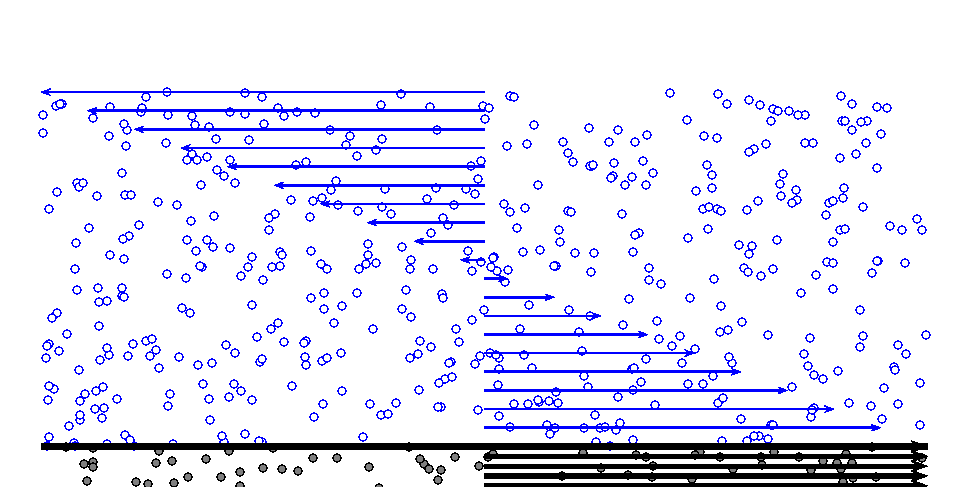
\includegraphics[width=0.5\textwidth]{adaptiveShearForce.pdf}
\caption{Velocities of solvent (blue) and wall particles (grey), shown as arrows.\label{fig:adaptShear}}
\end{figure}

In order to correct this, all particles close to the boundary, i.e. $h < r_{ shear}$, experience a tangential force:

\begin{equation} \label{eq:adaptive_shear_force}
F_t^k(h) = C_k\left(\Delta v_t \right) w(h)
\end{equation}

with $k$ as the iteration number and the weight function

\begin{equation} \label{eq:adaptive_sf_weight_fct}
w(h) = \left(1 - \frac{r}{r_{shear}} \right)^{power}
\end{equation}

and the iterative \textit{adaptive force strength}

\begin{equation} \label{eq:adaptive_force_strength}
C_{k+1} = C_k + \alpha \Delta v_t
\end{equation}

where $\alpha$ is the relaxation parameter, which is set in 'plane.dat'. This parameter could be calculated adaptively in future implementations.\\$\Delta v_t = v_t^{ BC} - v_t^{ est}$. The boundary's velocity is set in plane.dat, and the estimated velocity is extrapolated from the near-boundary velocity profile, which is obtained through local cell averaging.\\After a number of iterations, the particles' velocities approach the boundary's velocity ($\longrightarrow \Delta v_t \approx 0$) so that $F_t^k(h)$ and $C_k$ converge to constant values.\\
\\
\textit{Pressure force; forces read from external file} minimise disturbances in density profile. Particles close to a boundary experience an imbalance of forces, as each of them interacts with a not-fully spherical region of fluid particles, see graphics \ref{fig:wallNeighbours}.

\begin{figure}
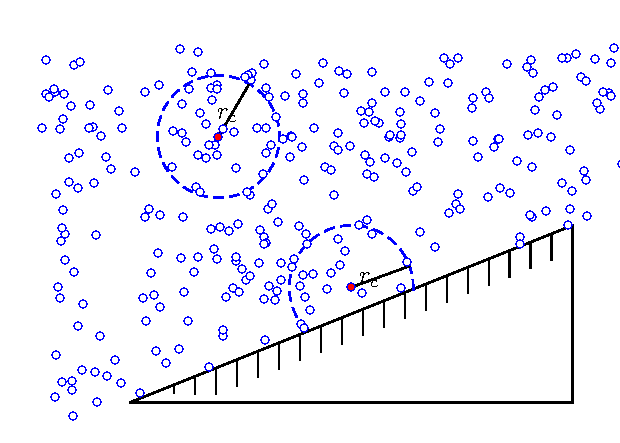
\includegraphics[width=0.5\textwidth]{wallNeighbours.pdf}
\caption{Interactions of solvent particle in bulk and of solvent particle close to wall.\label{fig:wallNeighbours}}
\end{figure}

This option does not consider wall particles and their interactions with the solvent/solute. It replaces the effect of wall particles with imposed conservative and dissipative forces calculated in advance and stored in an external file.\\The conservative force is calculated as:
\begin{equation}
\label{eq:wall_cons_force}
F_p(h) = -n \int_{V_s\backslash V_{ex}(h)} \frac{\partial U}{\partial r} g(r) dV
\end{equation}
with $V_s$ being the interaction sphere's volume, $V_{ex}(h)$ the volume excluded from the sphere by the boundary, and $g(r)$ is the radial distribution function of the specific fluid used in the simulation.


\subsection{fix\_wall\_force}
\label{sub:fix_wall_force}

This fix is the basic class for different LJ-Style walls (see \emph{fix\_wall\_lj126\_force}). It allows to define a wall parallel to one of the six simulation walls (xlo, xhi, ylo, yhi, zlo, zhi). In contrast to the original fix\_wall and its subfixes, this wall can either be fixed or it will move according to the forces acting on it. 

The force on the wall is divided in two parts:
\begin{align}
  F_\mathrm{wall} = F_\mathrm{push} + F_\mathrm{LJ}
\end{align}
where $F_\mathrm{push}$ is a parameter of the fix and $F_\mathrm{LJ}$ is the response force to the simulated system. In general, the wall will apply a force to every particle within its cutoff range perpendicular to the wall (the details of this force can be found in the subfix descriptions). The response force is the negative sum of all this forces. 

If the wall has a mass $m \neq 0$ (fix parameter), the wall will be moved in each timestep $\delta t$ by
\begin{align}
  x_{t+\delta t} = 2x_t - x_{t-\delta t} + \frac{1}{m} F_\mathrm{wall} \delta t^2,
\end{align}
where $x$ is the coordinate the wall is parallel to.

The quantities $F_\mathrm{LJ}$ and $x$ can be accessed through the local fix vector (see {\bfseries Examples} in \emph{fix\_wall\_lj126\_force}).


{\bfseries Syntax:}

This fix cannot be used directly.

\subsection{fix\_wall\_lj126\_force}
\label{sub:fix_wall_lj126_force}

The force between wall and system is given through the LJ-Energy
\begin{align}
  E = 4\epsilon \left[ \left(\frac{\sigma}{r}\right)^{12}  - \left(\frac{\sigma}{r}\right)^{6} \right] && r < r_c
\end{align}
where $r$ is the distance perpendicular to the wall. The force is given by $F_{LJ} = \sum\limits_{i=1}^N -\frac{\partial}{\partial r} E$ for every particle $1, \ldots, N$ within the cutoff radius $r_c$.


{\bfseries Syntax:}

\begin{lstlisting}
    fix ID group_ID wall/lj126/force coord $F_\mathrm{push}$ $m$ $\epsilon$ $\sigma$ cutoff
\end{lstlisting}

{\bfseries Examples:}

Create a lower and an upper wall in $z$-direction. The position of the lower wall is fixed (through $m=0$) while the upper wall is pushed with $F_\mathrm{wall} = -100$ and has a mass of $m=1000$ (all simulation units). The starting positions are the box limits in $z$-direction. The cutoff is chosen in such a way, that the wall is only repulsive.

\begin{lstlisting}
    fix walllo all wall/lj126/force zlo 0.0 0.0 1.0 1.0 1.12
    fix wallhi all wall/lj126/force zhi -100.0 1000.0 1.0 1.0 1.12
\end{lstlisting}

Access the reaction force $F_\mathrm{LJ}$ and the position $x$ of this walls and log them to a file \emph{dumpfile.force} every $1000$ steps:

\begin{lstlisting}[mathescape=false]
  variable force_lo equal f_walllo[1]
  variable force_hi equal f_wallhi[1]
  variable position_lo equal f_walllo[2]
  variable position_hi equal f_wallhi[2]
  fix wall_dump all print 1000 "${force_hi} ${force_lo} ${position_hi} ${position_lo}" file dumpfile.force title "# force_hi force_lo position_hi position_lo" screen no

\end{lstlisting}